The next step was to investigate the pluggable circuit board, the process and results of which are discussed in this section.

\subsection{Circuit board macro-analysis}
The circuit board itself was identified as a product of AMD, housing a 500 MHz AMD Geode LX800 and 256 MB DDR DRAM (Figure~\ref{fig:circuit-board}). Such technology was not believed to exist at the time, and it seems that great efforts have been devoted to keep this technology hidden.


\begin{figure}[h]
    \centering
    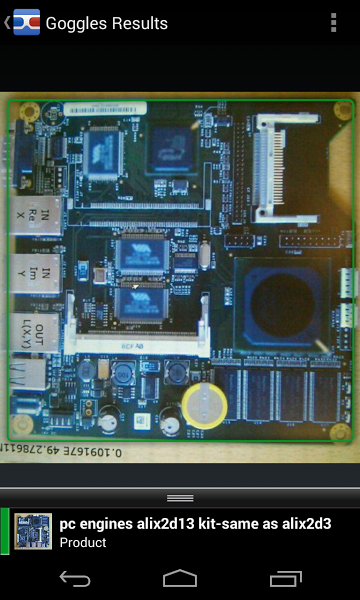
\includegraphics[width=0.8\columnwidth]{img/circuit-board.png}
    \caption{The identified circuit board}
    \label{fig:circuit-board}
\end{figure}

This leaves investigating yet another set of geographic coordinates: $0.109167E \; 49.278611N$. Learning from their previous experience, the geographic team decided to book a flight this time. They, of course, did not learn from their \emph{other} mistake, and hence spent quite some time travelling instead of taking the more sensible option of employing a parallel depth first search on the earth's map. The fact was reflected appropriately in their performance review. But we digress \ldots

\begin{figure}[h]
    \centering
    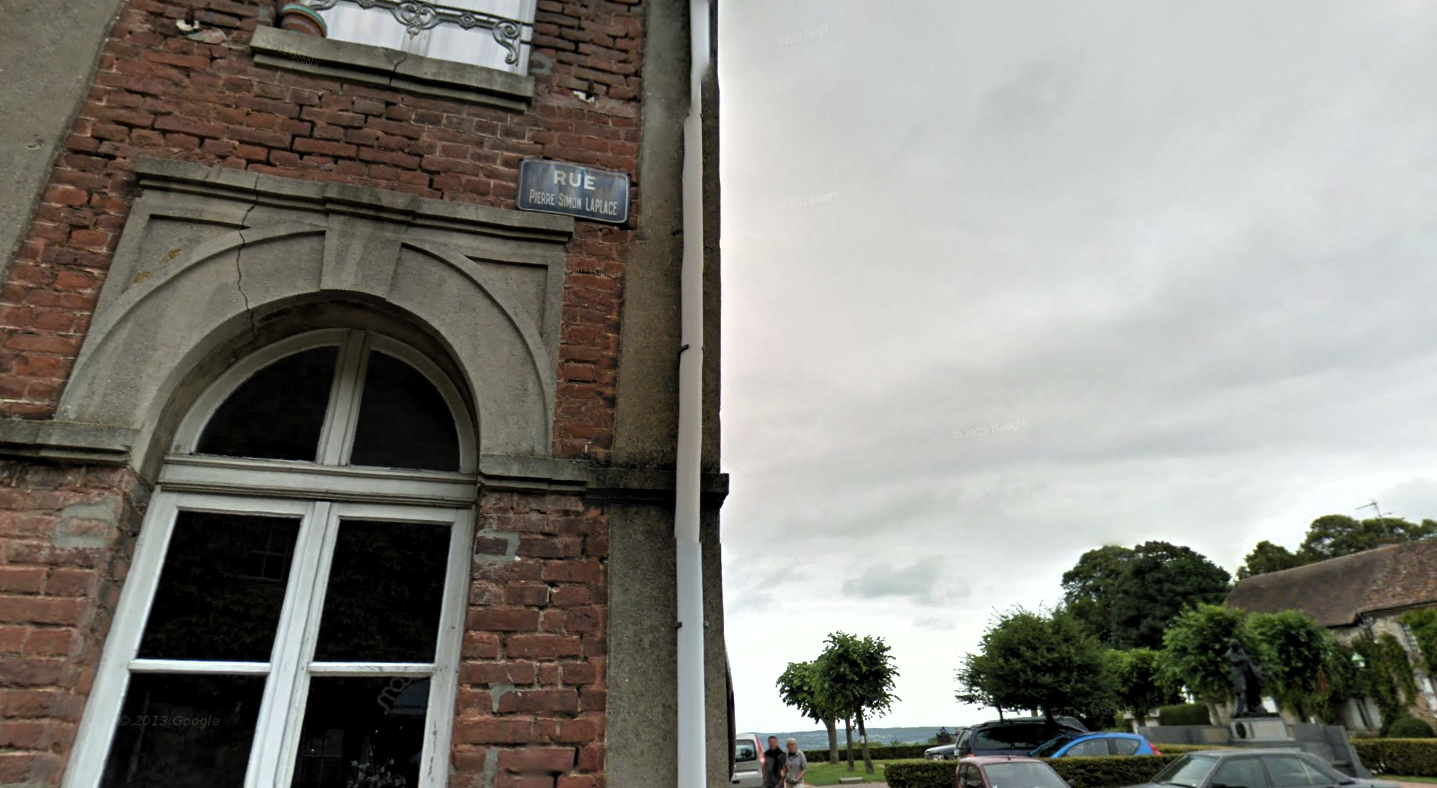
\includegraphics[width=0.95\columnwidth]{img/laplace-road.png}
    \caption{Rue Pierre Simon Laplace Road - You will never find a more blessed hive of charm and harmony}
    \label{fig:laplace-road}
\end{figure}


After an expensive trip to France, it was determined that the site referred to ``Ecole Beaumont en auge'' at ``Rue Pierre Simon Laplace Road'' (Figure~\ref{fig:laplace-road}). The connection was made the following week, when the team realised that the circuit was meant to employ some form of Laplace transform.


\subsection{Circuit board microanalysis}

With the macro analysis out of the way, our experts studied the circuit board's functionality through means of the reconstructed \texttt{mystery.o} object file.



\subsubsection{\texttt{strings} analysis}
Executing \texttt{strings} analysis on \texttt{mystery.o} revealed the following hidden data:

\begin{quote}
\texttt{(C) 2006 Svenska Aeroplan AB (SAAB) Designad av Margarita Gonz\'{a}lez Sampayo, Linkoping}
\end{quote}

The English translation:
\begin{quote}
\texttt{(C) 2006 Swedish Aeroplane Company Limited (SAAB) Designed by Margarita Gonz\'{a}lez Sampayo, Linkoping}
\end{quote}


A background search revealed that Dr. Margarita Holmberg (Gonz\'{a}lez Sampayo was her maiden name) had centred her PhD thesis\footnote{Engineering problem solving
- The case of the Laplace transform as a difficulty in learning in electric circuits and as a tool to solve real world problems} around the Laplace Transform in electric circuits. Indeed, it seems that SAAB is mentioned twice in her thesis, in the context of a practical application of the Laplace transform:

\begin{quote}
To solve problems working in Companies applying automatic control (for example, working in SAAB with aircraft dynamics) you use the Laplace transform.
\end{quote}




\subsubsection{\texttt{objdump} analysis}
The symbol table of \texttt{mystery.o} was extracted using \texttt{objdump --syms}. This revealed a number of interesting library functions being used:
\begin{itemize}
\item Mathematical functions, often operating on complex numbers, such as \texttt{cexp}, \texttt{muldc3}, \texttt{log}, and others.
\item Time-related functions, \texttt{time}, \texttt{strftime}, \texttt{strtol}, and \texttt{localtime})
\end{itemize}

Whilst the mathematical functions were to be expected, the time-related functions came as a surprise to our agents. This discovery motivated further, more dynamic, investigation.


\subsubsection{\texttt{ltrace} analysis}
By running \texttt{ltrace} whilst running the team obtained the library calls used during the computation phase. The first and subsequent runs are almost identical, apart from an extra initialisation step. The initialisation step includes a call to \texttt{localtime}, protected by \texttt{cxa\_guard} calls, which are used ``to support thread-safe, one-time initialisation of function scope variables''\footnote{\url{http://www.opensource.apple.com/source/libcppabi/libcppabi-14/src/cxa_guard.cxx}} (Figure~\ref{fig:l-calls}).


\begin{figure}[h]
    \centering

    \begin{tabular}{cc}
    \toprule
    Initial call & Subsequent calls \\

    \midrule

    \texttt
        time                                    & time        \\
        {\color{red} \_\_cxa\_guard\_acquire }  &             \\
        {\color{red} localtime }                &             \\
        {\color{red} \_\_cxa\_guard\_release }  &             \\
        strftime                                & strftime    \\
        strftime                                & strftime    \\
        strtol                                  & strtol      \\
        strtol                                  & strtol      \\
        \_\_muldc3                              & \_\_muldc3  \\
        cexp                                    & cexp        \\
        cexp                                    & cexp        \\
        \_\_divdc3                              & \_\_divdc3  \\
        \_\_muldc3                              & \_\_muldc3  \\
        \_\_muldc3                              & \_\_muldc3  \\
        sincos                                  & sincos      \\
        log                                     & log         \\
        cexp                                    & cexp        \\
        \_\_divdc3                              & \_\_divdc3  \\
        \_\_muldc3                              & \_\_muldc3  \\
        cexp                                    & cexp        \\
        \_\_muldc3                              & \_\_muldc3  \\
    \bottomrule
    \end{tabular}

    \caption{Trace of library calls for the initial and subsequent calls of the function \texttt{L()} . The extra library calls performed in the first function call are highlighted in red.}
    \label{fig:l-calls}
\end{figure}


\subsection{The Curious Case of \texttt{mystery.o}}

Our agent from the \emph{Hidden special unit for reverse analysis and decompilation} was able to successfully decompile the mysterious \texttt{mystery.o} file and write the equivalent C++ code. Further testing combined with the latest research in the field of \emph{Reasoning about programs} confirmed that our code produces exactly the same results as the initial object file. Below are some of the pseudo-code function calls that are used to compute the final answer:

\begin{verbatim}
muldc0  = complex(arg1,arg2) * complex(arg1,arg2);
cexp0   = exp (complex(alpha * arg1, alpha * arg2);
cexp1   = exp (complex(beta  * arg1, beta  * arg2);
cexp2   = exp (complex(arg1  * -1 * (mins/5 + 0.25), 
                       arg2  * -1 * (mins/5 + 0.25)));
[...]
multdc4 = complex(real(divdc1), imag(divdc1)) * 
          complex(real(cexp3) , imag(cexp3));
result  = compelx(real(muldc1) + real(muldc2) - real(muldc3) - real(muldc4),
                  imag(muldc1) + imag(muldc2) - imag(muldc3) - imag(muldc4));

\end{verbatim}

We would like to report some anomalies we have detected in the file, which we believe were put in place by the circuit designer in order to make the disassembly process more difficult:
\subsubsection{Extra strings}
We have noticed two ambiguous strings written at the beginning of the file:
\texttt{(C) 2006 Svenska Aeroplan AB (SAAB) Designad av Margarita Gonz\'{a}lez Sampayo, Linkoping}
\texttt{(C) 2006 Swedish Aeroplane Company Limited (SAAB) Designed by Margarita Gonz\'{a}lez Sampayo, Linkoping}
They provide some insights into who wrote the initial software and the year it might have been written.
\subsubsection{Computing $y = x^{782768}$, where $x = 0.999 \ldots$}
Due to the fact that $0.999 \ldots < 1$ and floating point numbers can't be represented exactly, the result of this exponentiation will be approximately $0$.
\subsubsection{Standard library functions: \\ \texttt{sincos(x)} and \texttt{log(x + 1)}}
The argument for the \texttt{sincos} function is $y$, the argument for the \texttt{log} function is $(y + 1)$, where $y$ is the result of the multiplication discussed above. Because $y \approx 0$, \texttt{sincos(y)} returns $(0,1)$ and \texttt{log(y+1)} returns $0$.
\subsubsection{Bogus while loops}
During the research phase, our agent has identified four repetitive structures. One repetitive structure is used to compute $y = x^{782768}$ in a very ineffective way. The other two repetitive structures have the same implementation and they serve as iterators through the two initial strings defined in the program. Their main purpose is to compute the offset between a specific \texttt{ASCII} character \texttt{( 0x80 )} and the initial strings. Due to the fact that the strings are hard-coded, the results computed by both the strings will always be \texttt{35 ( 0x23 )} and \texttt{49 ( 0x31 )}.
Lastly, the 4th structure is the \texttt{main} while loop. Its loop condition is:
$$49 + 35 + sin(y) + cos(y) + log(1+y) - 29 - 48 + y > 20$$

This simplifies to:
$$7 + sin(y) + cos(y) + log(1+y) > 20$$
Because y is a constant (0), $log(1+y) + sin(y) + cos(y)$ will be 1, so the loop condition $(8 > 20)$ will never be true.

Our agent is not sure whether these assembly artifacts and a lot of hard-coded values have been inserted in order to trick us or the compiler just generated general purpose code.

\subsubsection{Compiler (ab)uses the stack base pointer \texttt{(RBP)}}
During the analysis, it has been found that the \texttt{L()} function does not properly set the stack base pointer and instead it uses it as a general purpose register. This implies the fact that new variables are not created on the stack. The compiler is aware at compile time of the total number of variables used in the program and this is a known technique used by compilers in such situations.

\subsubsection{Closing remarks}
During the decompilation process our agent has used a test-driven approach, by writing scripts that would automate testing our computed function against the original \texttt{mystery.o} one. We used the program \textbf{faketime} in order to generate 1440 tests cases: 1 test for each minute of the day. Then we used a parallel diff program that would call both our function and the original \texttt{L()} one with different parameters and report any different results. Part of the tools used by the agent were the GNU Debugger \text{(gdb)}, with the peda plugin and the IDA program. No automated decomompilation tools have been used (because there are none for 64-bit programs).
